\documentclass[11pt]{article}
\usepackage[a4paper,margin=22mm,headheight=14pt]{geometry}
\usepackage{fontspec,graphicx}
\usepackage[unicode,hidelinks]{hyperref}
\setmainfont{Linux Libertine O}[Ligatures=TeX]
\graphicspath{{../source/presentation/}}
\hypersetup{pdftitle={S02 v002: critical notes and source limitations},pdfauthor={Digital transcription project; modern editorial apparatus}}
\setlength{\parindent}{0pt}
\setlength{\parskip}{6pt}
\linespread{1.08}
\tracinglostchars=2
\begin{document}
{\LARGE Critical notes and source limitations\par}
{\large S02 · v002 · Part I, printed pages 1–30\par}
\medskip
This apparatus is \texttt{MODERN\_EDITORIAL}. It is separate from Nallino’s historical Latin translation and notes. It records what the supplied scan supports; no new target-language translation or Arabic canonical correction is issued.

The reader preserves printed wording, numerals, note calls and source-line divisions. Irregularities are not silently harmonized. Three damaged character objects are preserved as exact source images within otherwise editable text or tables. Their unresolved interpretation does not mean that the source object has been omitted.
\section*{Unresolved character readings}

\subsection*{S02-U001 · Table}
{\small Printed p. 7; \texttt{AB01-PDF0096-T01-R04-C10}\par}
1 followed by a damaged digit, retained as source image.
\begin{center}
\includegraphics[height=7mm]{AB01-PDF0096-T01-R04-C10.png}\par{\small Enlarged source fragment; no reconstructed strokes.}\end{center}
12 is plausible from the surviving strokes; no numeric reading accepted. The CSV/TSV has an image marker, not 12.
{\small Certainty: high for pixel preservation; unresolved character reading.\par}
\subsection*{S02-U002 · Formula}
{\small Printed p. 12; \texttt{AB01-PDF0101-notes\_right-L003}\par}
59°3[damaged digit]′ within the numerator, retained as source image.
\begin{center}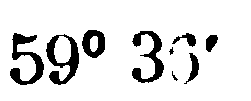
\includegraphics[height=7mm]{AB01-PDF0101-G01.png}\par{\small Enlarged source fragment; no reconstructed strokes.}\end{center}
59°36′ / 59°35′; 36 is supported by the body reading, but not imposed on the damaged note. No arithmetic correction; printed 72°2′ and 36°1′ retained.
{\small Certainty: high for exact image; minute digit unresolved.\par}
\subsection*{S02-U003 · Reading}
{\small Printed p. 18; \texttt{AB01-PDF0107-notes\_right-L017}\par}
Damaged Arabic spelling following corruptum.
\begin{center}
\includegraphics[height=7mm]{AB01-PDF0107-G01.png}\par{\small Enlarged source fragment; no reconstructed strokes.}\end{center}
No defensible complete character transcription assigned; exact image is the diplomatic object. No modern place-name substituted.
{\small Certainty: high for pixels; character interpretation withheld.\par}
\newpage\section*{Printed discrepancies and copy evidence}
\subsection*{S02-C001 · Reading}
{\small Printed p. 16; \texttt{AB01-PDF0105-body-L035}; \texttt{AB01-PDF0105-body-L038}\par}
78°23′ in the first statement; 78°28′ in the repeated value. Both are printed; no harmonization selected. The following 11°32′ is also retained. No emendation propagated.
{\small Certainty: high.\par}
\subsection*{S02-C002 · Reading}
{\small Printed p. 16; \texttt{AB01-PDF0105-body-L040}; \texttt{AB01-PDF0106-body-L001}\par}
Page 16 ends umbrae; page 17 begins brae rerum rotabunt. Apparent repeated ending across the physical seam. No deletion or joining of the repeated ending.
{\small Certainty: high.\par}
\subsection*{S02-C003 · Reading}
{\small Printed p. 10; \texttt{AB01-PDF0099}\par}
Two body calls printed (1); the second bottom note is numbered (2). No replacement of the second body call with (2). Original note call and note heading both retained.
{\small Certainty: high.\par}
\subsection*{S02-P001 · Provenance}
{\small Printed p. 17; \texttt{AB01-PDF0106-notes\_right-L002}\par}
Printed p.230 has an apparent overstrike on the holding-copy scan. Copy-specific marking; not attributed to Nallino as an authorized correction. Underlying 230 remains in the historical transcription.
{\small Certainty: mark visible; agency not established.\par}
\section*{Editorial scope and source}
The 30 source pages were read against the supplied page images. Native-resolution crops were used for difficult readings and the two diagrams. Existing embedded text served only as a comparison aid; no new OCR was run. The table cells are literal transcriptions, not regenerated arithmetical patterns.

The machine-readable ledgers supply stable source anchors, source-image rectangles where applicable, image hashes, table coordinates, marginal dispositions and the current checkpoint. Ordinary text-line anchors identify source page, region and ordinal; they are not asserted to be pixel-exact line boxes. References to Arabic pages printed by Nallino are recorded as locators, not as completed collation with an Arabic canonical edition.

This is a partial S02 candidate: printed pp. 31–109 are not transcribed here. Build and checking receipts accompany the package. They distinguish source reading from technical validation and do not claim an external human or separate-model review.

\medskip
{\small Nallino, C. A. (Ed. \& Trans.). (1903). \textit{Al-Battānī sive Albatenii opus astronomicum: Pars prima. Versio capitum cum animadversionibus}. Ulrich Hoepli. Controlling witness: SRC01, physical PDF pp. 90–119.\par}
\end{document}
